\documentclass[journal=jpclcd,manuscript=article]{achemso}

\usepackage[version=3]{mhchem} % Formula subscripts using \ce{}
\usepackage[T1]{fontenc}       % Use modern font encodings

\newcommand*\mycommand[1]{\texttt{\emph{#1}}}

\author{Authors}
\altaffiliation{Huygens-Kamerlingh Onnes Laboratory, Leiden University, RA, Leiden, The Netherlands}
\email{corresponding_author@physics.leidenuniv.nl}
\title[]
{Electrochemsitry of single Azurin shows time variant turnovers}

\abbreviations{IR,NMR,UV}
\keywords{American Chemical Society, \LaTeX}

\begin{document}

%%%%%%%%%%%%%%%%%%%%%%%%%%%%%%%%%%%%%%%%%%%%%%%%%%%%%%%%%%%%%%%%%%
%%%%%%% Start the main part of the manuscript here.%%%%%%%%%%%%%%
%%%%%%%%%%%%%%%%%%%%%%%%%%%%%%%%%%%%%%%%%%%%%%%%%%%%%%%%%%%%%%%%%%

\section{Introduction}
Introduction here.
%%%%%%Results and Discussion%%%%%%%%%
\section{Results and discussion\label{sec:results}}
Results and discussion.
\begin{scheme}
	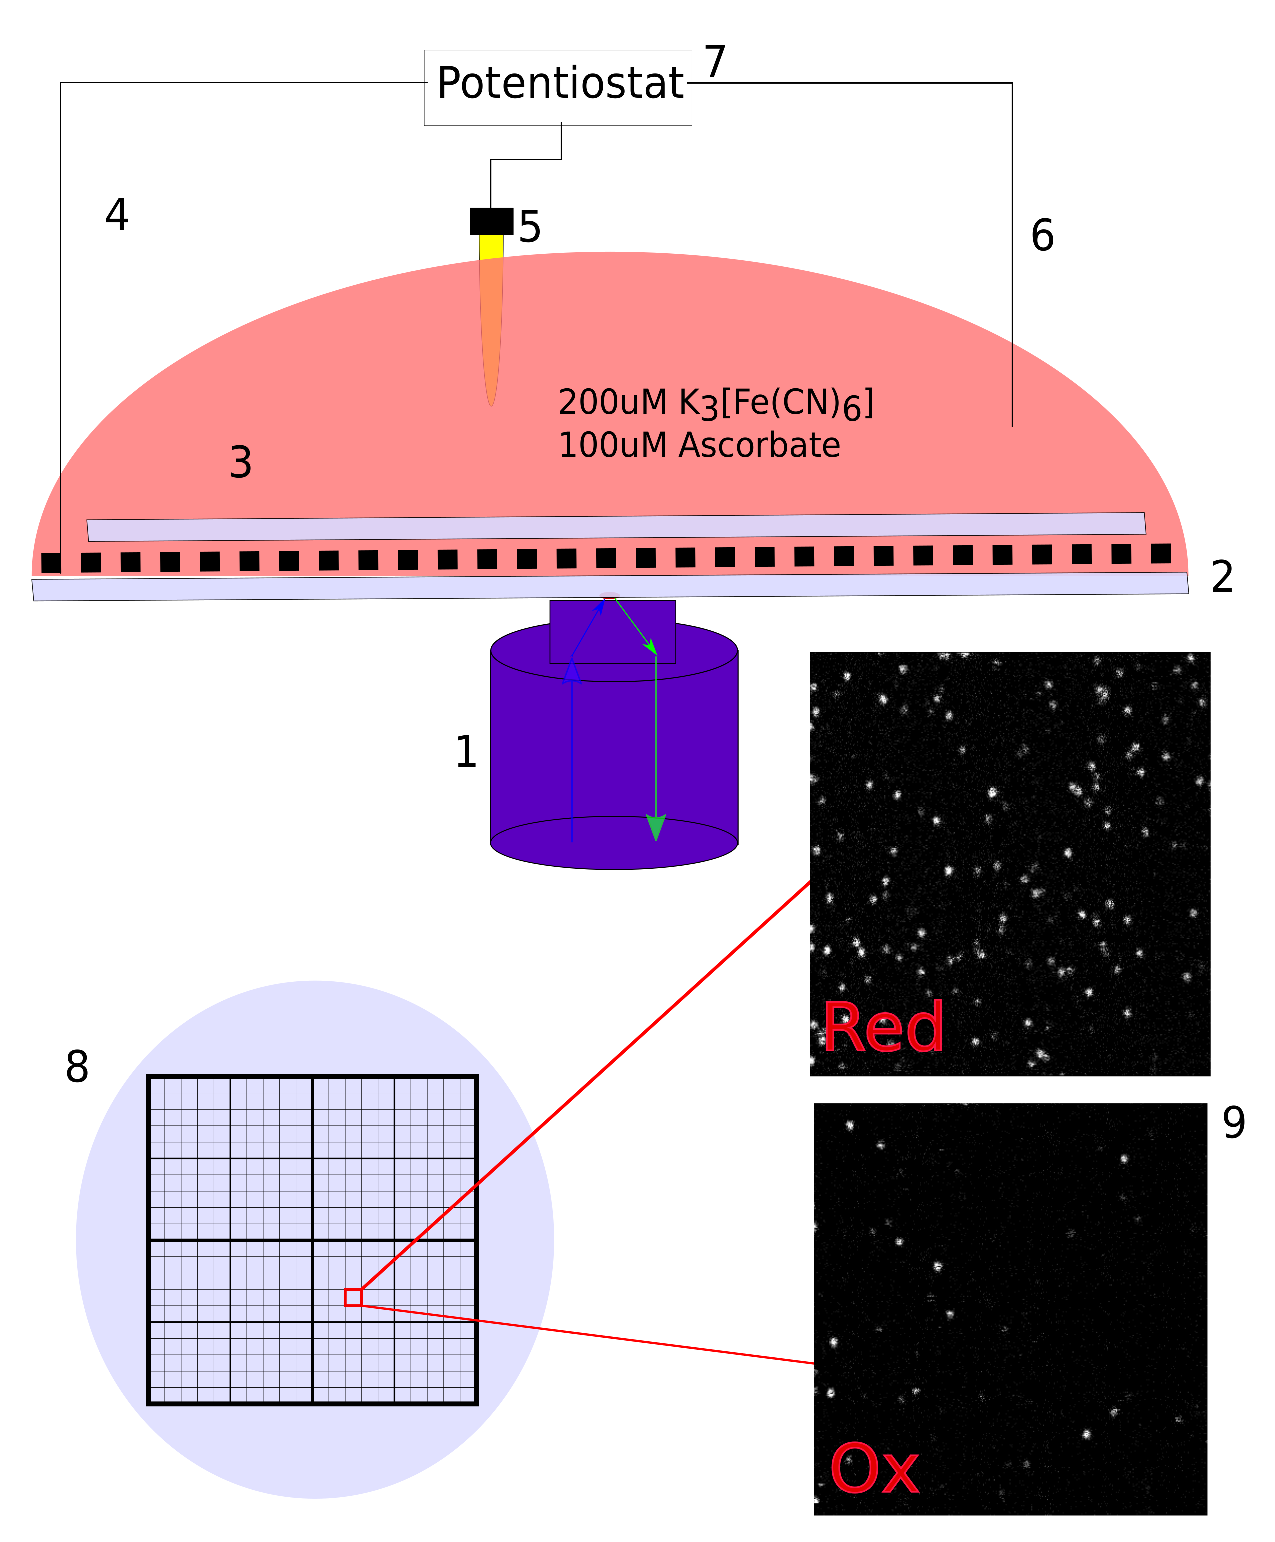
\includegraphics[scale=0.5]{Figure/Scheme_1_setup.eps}
	\caption{The scheme for}
  	\label{sch:setup}
\end{scheme}
%time trace
\begin{figure}
	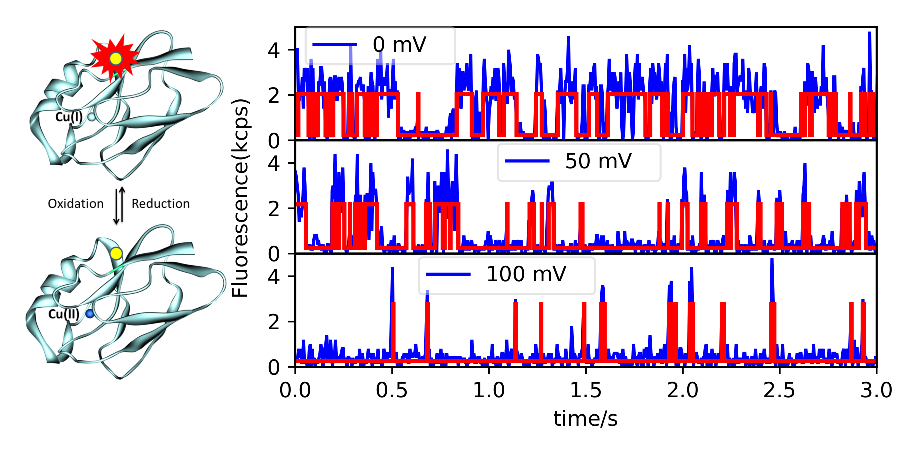
\includegraphics[width=\textwidth]{Figure/Figure_1_timetrace_CuAzu.eps}
	\caption{Time traces of labeled Cu-Azurin at different 		 		potential}
	\label{fig:timetrace}
\end{figure}
%Midpoint histogram
\begin{figure}
	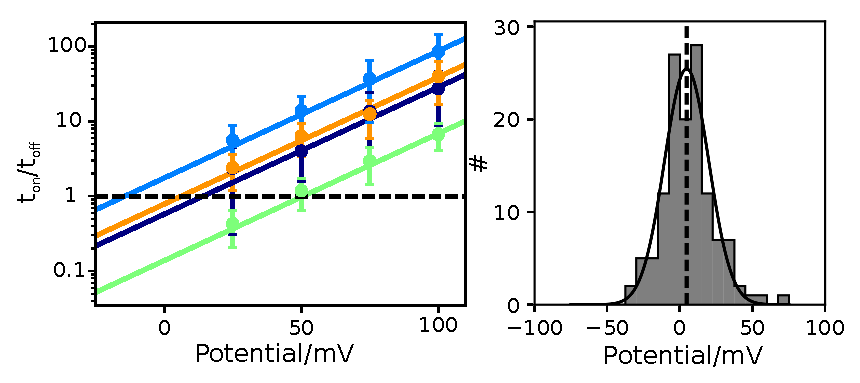
\includegraphics[width=\textwidth]{Figure/Figure_2_midpoint.eps}
	\caption{Ratio between on/off time as a function of Potential 		for each single molecule. The right plot is the histogram of  	 	midpoint potentials for 110 molecules}
	\label{fig:midpoint}
\end{figure}
%on-off 1D histogram
\begin{figure}
	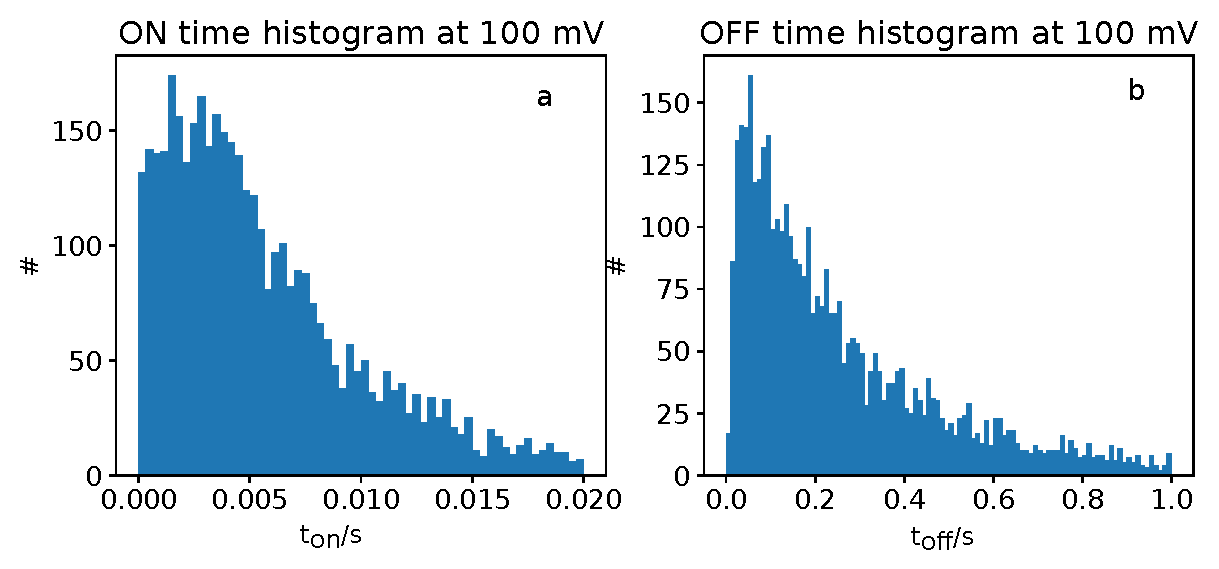
\includegraphics[width=\textwidth]{Figure/Figure_3_on_off_1D.eps}
	\caption{On off histogram}
	\label{fig:midpoint}
\end{figure}
%%%%%Experimental Section%%%%%%%%%%

\section{Experimental}
\bibliography{Azurin-SMredox}
\end{document}
